\documentclass[11pt]{article}
\usepackage[margin=1in]{geometry}
\usepackage{amsmath,amssymb,amsthm}
\usepackage{graphicx}
\usepackage{microtype}
\usepackage[colorlinks=true,linkcolor=blue,citecolor=blue,urlcolor=blue]{hyperref}

\newtheorem{proposition}{Proposition}

\title{The subproduct-system dimension question\\
was answered negatively}
\author{Run \texttt{fa\_banach\_001}, lane 17
  (\texttt{agent\_lane\_17})}
\date{13 August 2026}

\begin{document}
\maketitle

\begin{center}
\fbox{\parbox{0.91\textwidth}{
\textbf{Status: literature already answered (full negative answer).}
Gerhold--Skeide's Corollaries 5.5--5.6 give an explicit obstruction and
counterexample to the question of Shalit--Solel.
}}
\end{center}

\section{Exact source question}

Shalit and Solel define subproduct systems and, in Section 6.2 of
arXiv:0901.1422v3, ask whether every function
$f:\mathbb N\to\mathbb N$ satisfying
\begin{equation}\label{eq:submult}
 f(m+n)\le f(m)f(n)\qquad(m,n\in\mathbb N)
\end{equation}
is realized by a subproduct system $X$ with
$\dim X(n)=f(n)$ for all $n$.  The question is on printed/PDF page 35:
\begin{center}

\includegraphics[width=0.97\textwidth]{figures/source_question_crop.png}
\end{center}

The inequality \eqref{eq:submult} is plainly necessary because a subproduct
system has an isometric coproduct map
$X(m+n)\hookrightarrow X(m)\otimes X(n)$.  The question is whether it is
sufficient.

\section{The later answer}

Gerhold and Skeide prove in Theorem 3.15 of arXiv:1402.0198v2 that a sequence
$(d_n)_{n\ge0}$ is the dimension sequence of a finite-dimensional discrete
subproduct system if and only if it is the cardinality sequence of a word
system, also called a factorial language.  Corollary 5.5 then gives the
strictly stronger necessary family
\begin{equation}\label{eq:shifted}
 d_{m+n+k}\le d_{m+k}d_{n+k}
 \qquad(m,n,k\in\mathbb N).
\end{equation}
In particular,
\begin{equation}\label{eq:square}
 d_{k+1}\le d_k^2\qquad(k>0).
\end{equation}
Their immediately following Corollary 5.6 explicitly concludes that not
every submultiplicative sequence is realizable.  Both statements and their
counterexample appear on printed/PDF page 14:
\begin{center}
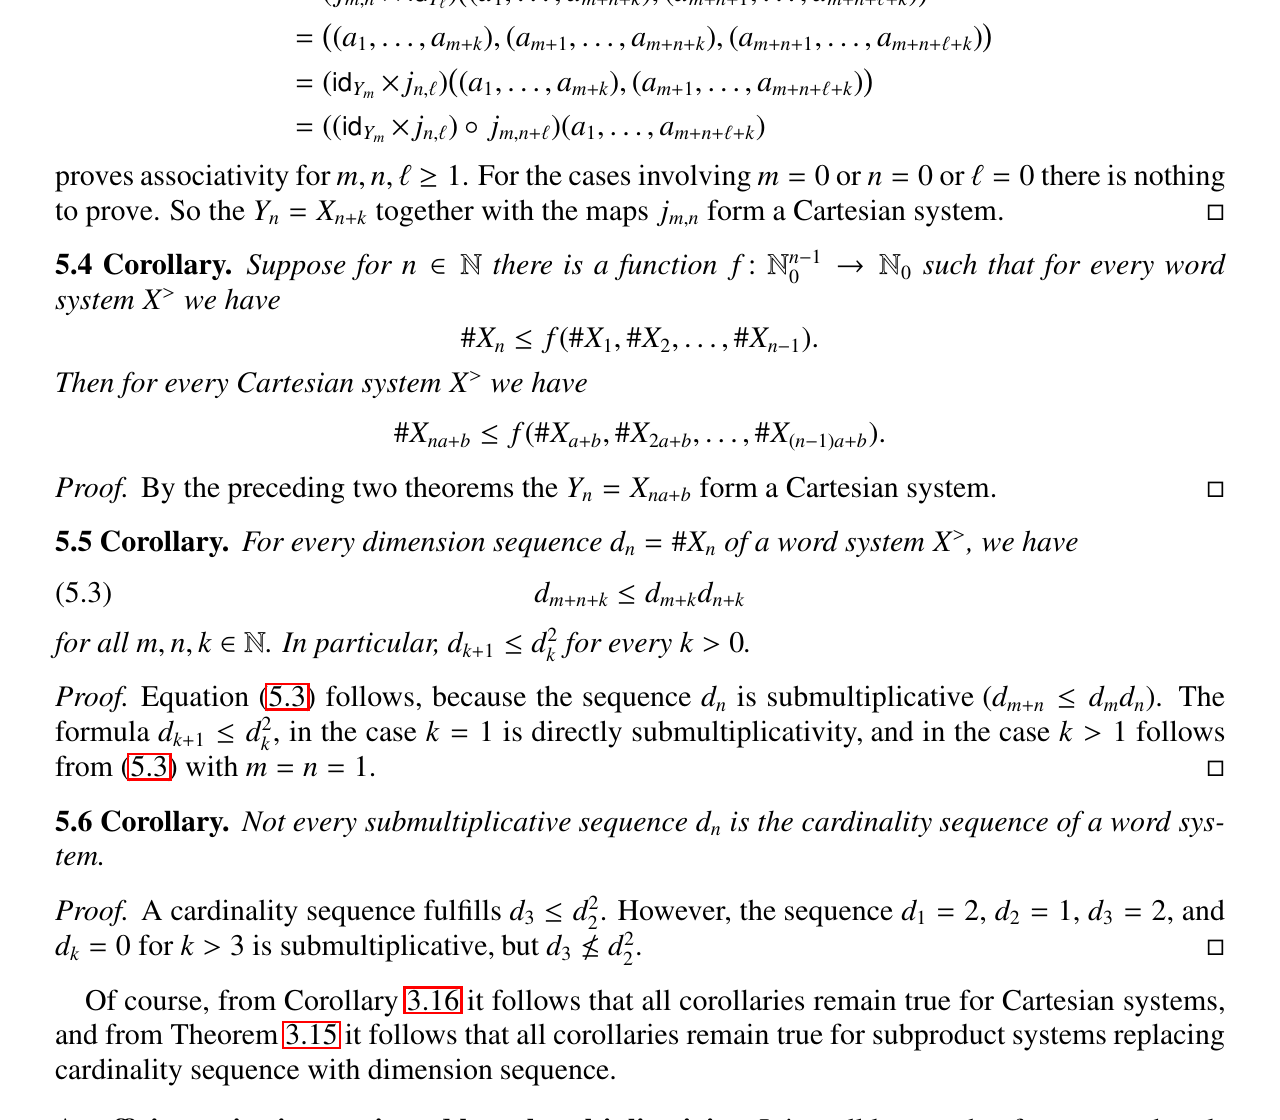
\includegraphics[width=0.97\textwidth]{figures/supporting_answer_crop.png}
\end{center}

Thus the answer to the source question is \emph{no}.

\section{Proof intuition and exact verification}

For a factorial language, let $W_j$ be its set of admitted words of length
$j$, so $d_j=|W_j|$.  Every admitted word of length $m+n+k$ determines two
overlapping admitted factors: its first $m+k$ letters and its last $n+k$
letters.  The two factors overlap in exactly $k$ letters, so together they
recover the original word.  Hence
\[
 W_{m+n+k}\longrightarrow W_{m+k}\times W_{n+k}
\]
is injective, proving \eqref{eq:shifted}.  The word-system/subproduct-system
dimension equivalence transfers this inequality to all subproduct systems.

The counterexample in Corollary 5.6 is
\[
 d_1=2,\qquad d_2=1,\qquad d_3=2,\qquad d_j=0\quad(j>3).
\]
It is submultiplicative: the only positive target terms beyond $d_1$ are
$d_2$ and $d_3$, and
\[
 d_2=1\le d_1^2=4,\qquad
 d_3=2\le d_1d_2=d_2d_1=2;
\]
every later target is zero.  But \eqref{eq:square} with $k=2$ would require
$2=d_3\le d_2^2=1$, a contradiction.

If $\mathbb N$ in the source question is interpreted as excluding zero in
the codomain, use instead
\[
 d_0=1,\quad d_1=2,\quad d_2=1,\quad d_3=2,\quad d_j=1\ (j\ge4).
\]
This sequence is positive and submultiplicative.  Indeed, sums $2$ and $3$
give exactly the two checks above, while every term at an index at least
four equals $1$ and every product on the right is at least $1$.  It still
violates $d_3\le d_2^2$.  The negative answer is therefore independent of
the convention for natural numbers.

\section{Provenance, scope, and review}

This is categorized as \emph{literature already answered}, not as a new
counterexample.  The later paper cites Shalit--Solel, studies exactly the
possible fiber-dimension sequences, proves their equivalence with factorial
language complexity sequences, and explicitly states the negative
submultiplicativity corollary.  The positive-tail modification above only
removes a harmless notation convention.

The result settles the yes/no realization question.  It does not classify
all realizable sequences; Gerhold--Skeide reduce that broader classification
to the generally open combinatorics of factorial languages.

The bounded status check covered the run indexes, the local parsed corpus,
exact question/phrase searches, and arXiv searches for subproduct systems,
dimension sequences, and submultiplicative sequences.  Human review need
only confirm the index convention and the transfer supplied by Theorem 3.15
of the supporting paper.

\begin{thebibliography}{9}
\bibitem{SS}
O.~M. Shalit and B.~Solel,
\emph{Subproduct systems}, Documenta Mathematica \textbf{14} (2009),
801--868; arXiv:0901.1422v3.

\bibitem{GS}
M.~Gerhold and M.~Skeide,
\emph{Subproduct systems and Cartesian systems; new results on factorial
languages and their relations with other areas},
Journal of Stochastic Analysis \textbf{1} (2020), no.~4, Article 5;
arXiv:1402.0198v2; doi:10.31390/josa.1.4.05.
\end{thebibliography}

\end{document}
